\begin{example}{Span as a subspace}
\begin{align*}
    W = \begin{Bmatrix}
    \begin{bmatrix}
    2s-5t\\3r+s-2t\\r-4s+3t\\-r+2s
    \end{bmatrix}
        \in \mathbb{R}^4:\text{r, s and t are scalars}
    \end{Bmatrix}
\end{align*}
Written on parameterised vector form
\begin{align*}
    W =
    r \begin{bmatrix}
        0 \\ 3 \\1 \\ -1
    \end{bmatrix}
    +s\begin{bmatrix}
        2 \\ 1 \\ -4 \\ 2
    \end{bmatrix}
    +t\begin{bmatrix}
        -5 \\ -2 \\ 3 \\ 0
    \end{bmatrix}
\end{align*}
\begin{align*}
    \mathcal{S}=
    \begin{Bmatrix}
    \begin{bmatrix}
        0 \\ 3 \\1 \\ -1
    \end{bmatrix}, 
    \begin{bmatrix}
        2 \\ 1 \\ -4 \\ 2
    \end{bmatrix},
    \begin{bmatrix}
        -5 \\ -2 \\ 3 \\ 0
    \end{bmatrix}
    \end{Bmatrix}
\end{align*}
Hence the span $\mathcal{S}$ is a subspace of $\mathbb{R}^4$
\end{example}


\begin{theorem}{Invertible Matrix P} \label{the:PMatrix}
    If an $m \times n$ matrix $A$ has a reduced row echelon form $R$, there will exist an invertible $m \times m$ elementary matrix $P$ which when multiplied with $A$ will equal $R$, such as
    \begin{align*}
        PA=R.
    \end{align*}
    \cite[127]{LiAl}
    \label{theo:invertible}
\end{theorem}
A proof of Theorem \ref{theo:invertible} leads to a justification of why it is possible to reduce a matrix $A$ to a matrix $R$.
\begin{proof}{Invertible Matrix P}
    $P$ is an invertible matrix so $P[A\mathbf{b}]=[R\mathbf{c}]$, where $[R\mathbf{c}]$ is the reduced row echelon form of $[A\mathbf{b}]$. 
    Hence the following can be stated
    \begin{align*}
        [PA\;P\mathbf{b}]=P[A\;\mathbf{b}]=[R\;\mathbf{c}].
    \end{align*}
    As seen, the connection between $PA$, $P\mathbf{b}$ and $R\mathbf{c}$ is
    \begin{align*}
        PA=R \quad\text{and}\quad P\mathbf{b}=\mathbf{c},
    \end{align*}
    hence
    \begin{align*}
        A = P^{-1}R \quad \text{and} \quad \mathbf{b} = P^{-1}\mathbf{c}.
    \end{align*}
    If $\mathbf{v}$ is a solution for $A\mathbf{x}=\mathbf{b}$, then $A\mathbf{v}=\mathbf{b}$. Thereby it can be expressed that 
    \begin{align*}
        R\mathbf{v}=(PA)\mathbf{v}=P(A\mathbf{v})=P\mathbf{b}=\mathbf{c}.
    \end{align*}
    This shows that $\mathbf{v}$ is a solution of $R\mathbf{x}=\mathbf{c}$
    and as said, $P$ is invertible, and therefore the following must be true
    \begin{align*}
        A\mathbf{v}=(P^{-1}R)\mathbf{v}=P^{-1}(R\mathbf{v})=P^{-1}\mathbf{c}=\mathbf{b}
    \end{align*}
    and as seen above, $\mathbf{v}$ is a solution of $A\mathbf{x}=\mathbf{b}$. As proved, $A\mathbf{x}=\mathbf{b}$ and $R\mathbf{x}=\mathbf{c}$ have the same solutions for \textbf{x}. \qedsymbol
\end{proof}


gauss distribution
\section{Gaussian Distribution}
\begin{definition}{Gaussian Distribution}
    The Gaussian distribution of a variable $x$ dimension is given by
    \begin{align*}
        \mathcal{N}(x|\Bar{x}, \sigma^2)=\frac{1}{(2\pi\sigma^2)^{1/2}}\exp\left\{-\frac{1}{2\sigma^2}(x-\Bar{x} )^2\right\}
    \end{align*}
    Where $\Bar{x}$ is the mean of the data, $\sigma$ is the standard deviation of the data and $\sigma^2$ is the variance. \cite[24]{patternmachineleaning}
\end{definition}
\autoref{fig:normalDistribution} show a Gaussian distribution with a mean of 2 and a standard deviation of 1. It can be seen that the Gaussian distribution have a maximum at the mean and is symmetric around the mean. 
\begin{figure}[H]
    \centering
    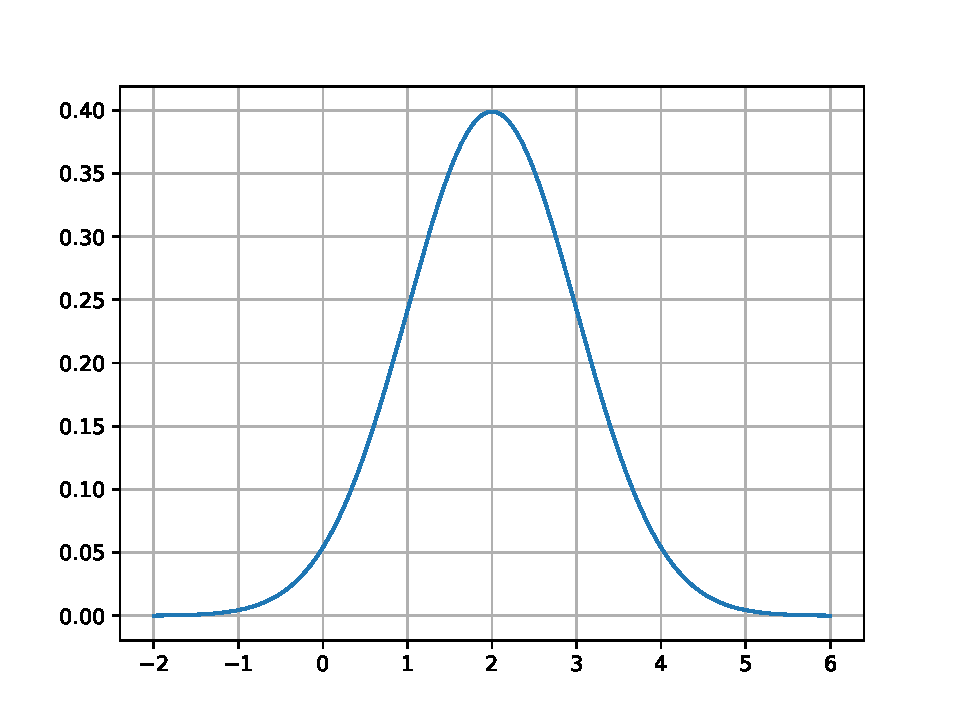
\includegraphics[width=0.8\textwidth]{figures/normalDistribution.pdf}
    \caption{A plot of a Gaussian distribution with a mean value of 2 and a standard deviation of 1.}
    \label{fig:normalDistribution}
\end{figure}
